\documentclass[10pt,a4paper,openright]{book}

%% Formateo del título del documento
\title{Topología elemental \\ Problemas}
\author{Íker Muñoz Martínez}
\date{}

\usepackage{silence}
%Disable all warnings issued by latex starting with "You have..."
\WarningFilter{latex}{You have requested package}
\usepackage{../style}

\begin{document}
\frontmatter
\maketitle
\setcounter{tocdepth}{3}% para que salgan las subsubsecciones en el indice
\tableofcontents

\mainmatter
\chapter{Lista 0: Para Empezar}%
\label{cha:lista0}

\section{Número 0.1}
\begin{enun}
Comprobar las leyes distributivas para la unión y la intersección de conjuntos, y las leyes de De Morgan.
\end{enun}
\begin{ej}
\begin{itemize}
\item Ley distributiva de la unión: $(A \cap B) \cup C = (A \cup C) \cap (B \cup C)$

$x \in (A \cap B) \cup C \Leftrightarrow (x \in A \wedge x \in B) \vee x \in C \Leftrightarrow (x \in A \vee x \in C) \wedge (x \in B \vee x \in C) \Leftrightarrow$ $x \in (A \cup C) \cap (B \cup C)$
\item Ley distributiva de la intersección: $(A \cup B) \cap C = (A \cap C) \cup (B \cap C)$

$x \in (A \cup B) \cap C \Leftrightarrow (x \in A \vee x \in B) \wedge x \in C \Leftrightarrow (x \in A \wedge x \in C) \vee (x \in B \wedge x \in C) \Leftrightarrow$ $x \in (A \cap C) \cup (B \cap C)$
\item Leyes de De Morgan: $(A \cup B)^c = A^c \cap B^c \ \& \ (A \cap B)^c = A^c \cup B^c$
\begin{enumerate}[label={(\arabic*)}]
\item $x \in (A \cup B)^c \Leftrightarrow x \notin A \cup B \Leftrightarrow x \notin A \wedge x \notin B \Leftrightarrow x \in A^c \wedge x \in B^c \Leftrightarrow x \in A^c \cap B^c$
\item $A \cap B = A^{cc} \cap B^{cc} \overset{(1)}{=} (A^c \cup B^c)^c$, y tomando complementarios en ambos lados obtenemos la segunda ley.
\end{enumerate}
\end{itemize}
\end{ej}

\section{Número 0.2}
\begin{enun}
Se consideran una aplicación $f: A \rightarrow B$ y subconjutos $A_0 \subset A, B_0 \subset B$.
\begin{enumerate}[label={(\arabic*)}]
 \item Demostrar que $A_0 \subset f^{-1}(f(A_0))$ y que se da la igualdad si $f$  es inyectiva.
 \item Demostrar que $f(f^{-1}(B_0)) \subset B_0$ y que se da la igualdad si $f$ es sobreyectiva.
\end{enumerate}
\end{enun}
\begin{ej}
\begin{enumerate}[label={(\arabic*)}]
 \item Sea $x \in A_0$. Así, $f(x) \in f(A_0)$, y por definición de preimagen, $x \in f^{-1}(f(A_0))$. En particular, obtenemos la igualdad $A_0 
 = f^{-1}(f(A_0))$ si $f$ es inyectiva. Supongamos que $\exists y \in f^{-1}(f(A_0)) \setminus A_0$. Así, $f(y) \in f(A_0)$, luego existe un $x \in A_0$ tal que $f(y) = f(x)$. Como $f$ es inyectiva, $x = y \in A_0$, lo que nos lleva a una contradicción. 
 \item Sea $y \in f(f^{-1}(B_0))$. Así, existe $x \in f^{-1}(B_0)$ tal que $y = f(x)$. Por tanto, si aplicamos f, obtenemos que $f(x) = y \in B_0$. En particular, obtenemos la igualdad $f(f^{-1}(B_0)) = B_0$ si $f$ es sobreyectiva. Si $y \in B_0$, como $f$ es sobreyectiva, existe un $x \in f^{-1} (B_0)$ tal que $f(x) = y$. Aplicamos $f^{-1}$ y obtenemos que $f^{-1}(y) = x \in f^{-1}(B_0)$, y al aplicar $f$ obtenemos $f(x) = y \in f(f^{-1}(B_0))$.
\end{enumerate}
\end{ej}

\section{Número 0.3}
\begin{enun}
Se consideran una aplicación $f: A \rightarrow B$ y colecciones de subconjutos $A_i \subset A, B_i \subset B$.
\begin{enumerate}[label={(\arabic*)}]
 \item Probar que $f^{-1}$ conserva inclusiones, uniones, intersecciones y diferencias
 \begin{enumerate}[label={(\alph*)}]
 \item Si $B_i \subset B_j$, entonces $f^{-1} (B_i) \subset f^{-1}(B_j)$
 \item $f^{-1}  (\bigcup_i B_i) = \bigcup_i f^{-1} (B_i)$
 \item $f^{-1}  (\bigcap_i B_i) = \bigcap_i f^{-1} (B_i)$
 \item $f^{-1} (B_i \setminus B_j) = f^{-1}(B_i) \setminus f^{-1}(B_j)$
 \end{enumerate}
 \item Demostrar que $f$ conserva solamente las uniones y las inclusiones:
 \begin{enumerate}[label={(\alph*)}]
 \item Si $A_i \subset A_j$, entonces $f (A_i) \subset f(A_j)$
 \item $f(\bigcup_i A_i) = \bigcup_i f (A_i)$
 \item $f  (\bigcap_i A_i) \subset \bigcap_i f(A_i)$; se da la igualdad si $f$ es inyectiva.
 \item $f (A_i \setminus A_j) \supset f(A_i) \setminus f(A_j)$; se da la igualdad si $f$ es inyectiva.
 \end{enumerate}
\end{enumerate}
\end{enun}
\begin{ej}
\begin{enumerate}[label={(\arabic*)}]
 \item Probar que $f^{-1}$ conserva inclusiones, uniones, intersecciones y diferencias
 \begin{enumerate}[label={(\alph*)}]
 \item Sea $x \in f^{-1}(B_i)$. Así, $f(x) \in B_i \subset B_j$, y por tanto, $x \in f^{-1}(B_j)$.
 \item Sea $x \in f^{-1}(\bigcup_i B_i) \Leftrightarrow f(x) \in \bigcup_i B_i \Leftrightarrow \exists i \in I : f(x) \in B_i \Leftrightarrow \exists i \in I : x \in f^{-1} (B_i) \Leftrightarrow x \in \bigcup_i f^{-1}(B_i)$.
 \item  Análogamente, sea $x \in f^{-1}(\bigcap_i B_i) \Leftrightarrow f(x) \in \bigcap_i B_i \Leftrightarrow \forall i \in I : f(x) \in B_i \Leftrightarrow \forall i \in I : x \in f^{-1} (B_i) \Leftrightarrow x \in \bigcap_i f^{-1}(B_i)$.
 \item  Sea $x \in f^{-1} (B_i \setminus B_j) \Leftrightarrow f(x) \in B_i \setminus B_j \Leftrightarrow f(x) \in B_i \wedge f(x) \notin B_j \Leftrightarrow x \in  f^{-1}(B_i) \wedge x \notin  f^{-1}(B_j) \Leftrightarrow x \in  f^{-1}(B_i) \setminus  f^{-1}(B_j)$.
 \end{enumerate}
 \item Demostrar que $f$ conserva solamente las uniones y las inclusiones:
 \begin{enumerate}[label={(\alph*)}]
 \item  Sea $x \in f(A_i)$. Entonces, $\exists a \in A_i : f(a) = x \Rightarrow a \in A_i \subset A_j$, luego $x = f(a) \in f(A_j)$.
 \item Sea $x \in f(\bigcup_i A_i) \Leftrightarrow \exists a \in \bigcup_i A_i : f(a) = x \Leftrightarrow \exists i \in I \ \exists a \in A_i : f(a) = x$. Por tanto, $\exists i \in I : f(a) \in f(A_i) \ \& \ f(a) = x  \Leftrightarrow f(a) \in \bigcup_i f(A_i) \ \& \ f(a) = x \Leftrightarrow x \in f\bigcup_i f(A_i)$.
 \item Veamos primero el contenido general, y después el caso en que $f$ es inyectiva.
 \begin{itemize}
 \item Sea $x \in f(\bigcap_i A_i)$. Entonces, $\exists a \in \bigcap_i A_i : f(a) = x \Rightarrow \forall i \in I \ \exists a \in A_i$, luego $\forall i \in I \ \exists f(a) \in f(A_i) \ \& \ f(a) =x$. Por tanto, $\forall i \in I x \in f(A_i)$, es decir, $x \in \bigcap_i f(A_i)$.
 \item (Si $f$ inyectiva) Sea $x \in \bigcap_i f( A_i)$. Entonces, $\forall i \in I : x \in f(A_i)$. Entonces, $\forall i \in I \ \exists a \in A_i : f(a) = x \Rightarrow \exists a \in \bigcap_i A_i : f(a) = x$, y como la $f$ es inyectiva, $x \in f(\bigcap_i A_i)$.
 \end{itemize}
 \item  Veamos primero el contenido general, y después el caso en que $f$ es inyectiva.
 \begin{itemize}
 \item Sea $x \in f(A_i) \setminus f(A_j)$, es decir, $x \in f(A_i) \wedge x \in f(A_j)^c$. Por tanto, $\begin{cases} \exists a \in A_i : f(a) = x \\ \nexists a \in A_j : f(a) = x  \end{cases}\Rightarrow \exists a \in A_i \cap A_j^c : f(a) = x$, es decir, $x \in f(A_i \setminus A_j)$.
 \item (Si $f$ inyectiva) Sea $x \in f(A_i \setminus A_j)$, es decir $\exists a \in A_i \setminus A_j : f(a)=x$. Por tanto, $\begin{cases} \exists a \in A_i : f(a) = x \\ \exists a \notin A_j : f(a) = x  \end{cases}$. Como $f$ es inyectiva, los $a$ son los mismos y por tanto $x \in f(A_i) \cap f(A_j)^c$, es decir, $x \in f(A_i) \setminus f(A_j)$.
 \end{itemize}
 \end{enumerate}
\end{enumerate}
\end{ej}

\section{Número 0.4}
\begin{enun}
Probar que el conjunto $\mathbb{Q}$ de los números racionales es numerable. Probar que el intervalo $[0,1]$ no es numerable, y que por tanto no lo es $\mathbb{R}$.
\end{enun}
\begin{ej}
\begin{enumerate}[label={(\arabic*)}]
\item Veamos primeramente que el conjunto $\mathbb{Q}$ es numerable. Apoyándonos en el hecho de que $\mathbb{Z}$ es numerable, construimos la siguiente aplicación: \begin{align*}
f: \mathbb{Z} \times \mathbb{Z}^* &\rightarrow \mathbb{Q} \\ 
(p,q) &\mapsto \frac{p}{q}
\end{align*}
La aplicación $f$ es sobreyectiva, ya que $\forall x \in \mathbb{Q}, \exists p,q \in \mathbb{Z} : x = \frac{p}{q}, q \neq 0$. Así, $$Card(\mathbb{Q}) \leq Card(\mathbb{Z} \times \mathbb{Z}) = Card(\mathbb{N})$$ Luego $\mathbb{Q}$ es numerable.
\item Para probar que el intervalo $[0,1]$ no es numerable, emplearemos el argumento conocido como \textit{diagonalización de Cantor}. Por reducción al absurdo, supongamos que el intervalo fuere numerable. Si lo fuera, admitiría una posible enumeración $\{r_n\}_n$. Cada uno de los elementos de la sucesión será un $x \in (0,1)$ (no afecta a la numerabilidad que quitemos los extremos, pues son únicamente dos puntos, es decir, un conjunto finito), que podemos expresar utilizando sus cifras decimales $x = 0.\ldots$ La sucesión tendría la pinta:
\begin{align*}
r_1 &= 0.a_1^1a_2^1a_3^1\ldots \\ 
r_2 &= 0.a_1^2a_2^2a_3^2\ldots \\ 
r_3 &= 0.a_1^3a_2^3a_3^3\ldots \\ 
r_4 &= 0.a_1^4a_2^4a_3^4\ldots \\ 
r_5 &= 0.a_1^5a_2^5a_3^5\ldots \\ 
&\vdots
\end{align*}
Cada $a_i^j$ es un número natural comprendido entre $0$ y $9$. Consideramos entonces el siguiente número: $$R= 0.r_1r_2r_3r_4 \ldots: r_i = a_i^i + 1 (\textsf{mod} 10)$$
El número $R$ pertenece al intervalo; no obstante, difiere con todos los $r_i$ en al menos una posición. Es decir, hemos construido un número que no se encuentra en la sucesión $\{r_n\}_n$, por lo que nuestra hipótesis de que el intervalo $[0,1]$ fuera numerable debe ser falsa.

Además, no es difícil comprobar que la aplicación 
\begin{align*}
f: (0,1) &\rightarrow \mathbb{R} \\
x &\mapsto \tan\left[\pi (x - \frac{1}{2})\right]
\end{align*}
Es una biyección. Por tanto, $\mathbb{R}$ no es numerable, y en particular, $Card(\mathbb{R}) = Card([0,1])$
\end{enumerate}

\end{ej}

\section{Número 0.5}
\begin{enun}
(Distancias en $\mathbb{R}^n$) Comprobar que cada una de las siguientes es una distancia en $\mathbb{R}^n$ y estudiar como son las bolas en cada una de ellas.
\begin{align*}
d(x,y) = \sqrt{\sum_i (x_i - y_i)^2} && \rho_1(x,y) = \sum_i | x_i - y_i| && \rho_2 (x,y) = \max_i |x_i -y_i|
\end{align*}
Para la primera, utilizar la \textit{desigualdad triangular} o \textit{de Minkowsky} $$\sqrt{\sum_i (a_i + b_i)^2} \leq \sqrt{\sum_i a_i^2} + \sqrt{\sum_i b_i^2}$$
\end{enun}
\begin{ej}
dgerhgsre
\end{ej}
\chapter{Lista 1: Espacios Topológicos}%
\label{cha:lista1}
\section{Número 1.1}
\begin{enun}
Sea $X$ un conjunto, y $\matheuler{T}_{CF}$ la familia de todos los subconjuntos de $X$ cuyo complementario es finito, más el conjunto vacío. Probar que $\matheuler{T}_{CF}$ es una topología en $X$. Esta topología se llama, por razones evidentes, \textit{topología de los complementarios finitos}. ¿Qué topología obtenemos si $X$ es un conjunto finito?
\end{enun}
\begin{ej}
Veamos que $\matheuler{T}_{CF}$ satisface las tres propiedades para que sea topología:
\begin{enumerate}[label={(\arabic*)}]
\item Por definición, $\emptyset \in \matheuler{T}_{CF}$. Además, $X^c = \emptyset$ es finito, por lo que $X \in \matheuler{T}_{CF}$.
\item Comprobemos que las uniones arbitrarias de elementos del $\matheuler{T}_{CF}$ están en $\matheuler{T}_{CF}$. Sean $U_i \in \matheuler{T}_{CF}$ con $i \in I$ arbitrario. Veamos entonces que $X \setminus \bigcup_{i \in I} U_i$ es finito.
$$X \setminus \bigcup_{i \in I} U_i \overset{De Morgan}{=} \bigcap_{i \in I}X \setminus U_i$$
Como los $U_i \in \matheuler{T}_{CF}$, su complementario es finito, y la intersección arbitraria de conjuntos finitos es finita. Así, $\bigcup_{i \in I} U_i \in \matheuler{T}_{CF}$
\item Finalmente, comprobemos que las intersecciones finitas de elementos de $\matheuler{T}_{CF}$ están en $\matheuler{T}_{CF}$. Basta comprobarlo para dos conjuntos $U, U'$, pues la intersección finita de conjuntos puede definirse dos a dos. Así, sean $U, U' \in \matheuler{T}_{CF}$, y veamos que $X \setminus (U \cap U')$ es finito.
$$X \setminus (U \cap U') \overset{De Morgan}{=} (X \setminus U) \cup (X \setminus U')$$
Como $U, U' \in \matheuler{T}_{CF}$, su complementario es finito, y la unión finita de conjuntos finitos es finita. Por tanto, $\bigcap_{i \in I} U_i : I $ finito $\in \matheuler{T}_{CF}$.
\end{enumerate}
En particular, si $X$ es finito, cualquier subconjunto suyo $A \subset X$ tiene complementario finito, y por tanto, pertenece a $\matheuler{T}_{CF}$. Así, en particular todos los puntos son abiertos, y por tanto, $\matheuler{T}_{CF} = \matheuler{T}_{Discreta}$.
\end{ej}


\section{Número 1.4}
\begin{enun}
Sea $X$ un conjunto infinito y $\matheuler{T}$ una topología en la que todos los conjuntos infinitos son abiertos. Demostrar que $\matheuler{T}$ es la topología discreta.
\end{enun}
\begin{ej}
La idea de la demostración consiste en utilizar la caracterización de la topología discreta, es decir, para ver que la topología es la discreta tenemos que ver que todos los puntos del conjunto son abiertos.

Como $X$ es infinito, existe una sucesión $\{x_n\}_{n \in \mathbb{N}}$ de elementos diferentes. Sea $A = \{x_1, x_2,x_3,\ldots \} \subset X$ cuyos elementos son los de la sucesión $x_n$. Como $A$ es infinito, por la definición de la topología, $A \in \matheuler{T}$, y además podemos descomponer de forma disjunta $A$ como la subsucesión de elementos con índice par y la subsucesión de elementos de índice impar:
$$A = A_1 \sqcup A_2 = \{x_i : i \ \mathsf{mod} \ 2 = 1\} \sqcup \{x_i : i\  \mathsf{mod} \ 2 = 0\}$$
Y además, por ser ambos infinitos, $A_1, A_2 \in \matheuler{T}$. Por ser $\matheuler{T}$, las intersecciones finitas de elementos de $\matheuler{T}$ están contenidas en $\matheuler{T}$, y también las uniones arbitrarias; así, dado $x \in X$ arbitrario:
$$\underbrace{(A_1 \cup \{x\})}_{\in \matheuler{T}} \cap \underbrace{(A_2 \cup \{x\})}_{\in \matheuler{T}} = \{x\} \in \matheuler{T}$$
Como $x$ es arbitrario, quiere decir que todos los puntos son abiertos, y por la caracterización, la topología ante la que nos encontramos es la discreta.
\end{ej}

\section{Número 1.7}
\begin{enun}
En el plano $X = \mathbb{R}^2$ se considera la familia $\matheuler{T}$ de todos los subconjuntos $U$ tales que para cada punto $(a,b) \in U$ existe $\varepsilon > 0$ con 
$$((a - \varepsilon, a + \varepsilon) \times \{b\}) \cup (\{a\} \times (b-\varepsilon, b + \varepsilon)) \subset U$$
Estudiar si $\matheuler{T}$  es una topología en $X$.
\end{enun}
\begin{ej}
Para comprobar que $\matheuler{T}$ es en efecto una topología, debemos comprobar que satisface las tres propiedades de la definición de topología. No obstante, antes de comenzar a demostrar, intentaremos tener una idea intuitiva de cómo son los abiertos en esta topología.
\begin{figure}[h]
\tikzset{every picture/.style={line width=0.75pt}} %set default line width to 0.75pt        

\begin{tikzpicture}[x=0.75pt,y=0.75pt,yscale=-1,xscale=1]
%uncomment if require: \path (0,300); %set diagram left start at 0, and has height of 300

%Shape: Polygon Curved [id:ds521474139569552] 
\draw   (135,31) .. controls (170,-13) and (282,26) .. (262,46) .. controls (242,66) and (277,104) .. (297,134) .. controls (317,164) and (166,174) .. (146,144) .. controls (126,114) and (100,75) .. (135,31) -- cycle ;
%Straight Lines [id:da9767797404673607] 
\draw [color={rgb, 255:red, 74; green, 144; blue, 226 }  ,draw opacity=1 ]   (169.53,45.25) -- (169.97,97.25) ;
\draw [shift={(170,100.25)}, rotate = 269.51] [fill={rgb, 255:red, 74; green, 144; blue, 226 }  ,fill opacity=1 ][line width=0.08]  [draw opacity=0] (10.72,-5.15) -- (0,0) -- (10.72,5.15) -- (7.12,0) -- cycle    ;
\draw [shift={(169.5,42.25)}, rotate = 89.51] [fill={rgb, 255:red, 74; green, 144; blue, 226 }  ,fill opacity=1 ][line width=0.08]  [draw opacity=0] (10.72,-5.15) -- (0,0) -- (10.72,5.15) -- (7.12,0) -- cycle    ;
%Straight Lines [id:da08757217471883894] 
\draw [color={rgb, 255:red, 74; green, 144; blue, 226 }  ,draw opacity=1 ]   (143.5,71.25) -- (197.5,71.25) ;
\draw [shift={(200.5,71.25)}, rotate = 180] [fill={rgb, 255:red, 74; green, 144; blue, 226 }  ,fill opacity=1 ][line width=0.08]  [draw opacity=0] (10.72,-5.15) -- (0,0) -- (10.72,5.15) -- (7.12,0) -- cycle    ;
\draw [shift={(140.5,71.25)}, rotate = 0] [fill={rgb, 255:red, 74; green, 144; blue, 226 }  ,fill opacity=1 ][line width=0.08]  [draw opacity=0] (10.72,-5.15) -- (0,0) -- (10.72,5.15) -- (7.12,0) -- cycle    ;
%Straight Lines [id:da42265688096601306] 
\draw [color={rgb, 255:red, 74; green, 144; blue, 226 }  ,draw opacity=1 ]   (433.5,90.25) -- (526.5,90.25) ;
\draw [shift={(529.5,90.25)}, rotate = 180] [fill={rgb, 255:red, 74; green, 144; blue, 226 }  ,fill opacity=1 ][line width=0.08]  [draw opacity=0] (10.72,-5.15) -- (0,0) -- (10.72,5.15) -- (7.12,0) -- cycle    ;
\draw [shift={(430.5,90.25)}, rotate = 0] [fill={rgb, 255:red, 74; green, 144; blue, 226 }  ,fill opacity=1 ][line width=0.08]  [draw opacity=0] (10.72,-5.15) -- (0,0) -- (10.72,5.15) -- (7.12,0) -- cycle    ;
%Straight Lines [id:da8106871969505601] 
\draw [color={rgb, 255:red, 74; green, 144; blue, 226 }  ,draw opacity=1 ]   (480,135.5) -- (480,43.5) ;
\draw [shift={(480,40.5)}, rotate = 90] [fill={rgb, 255:red, 74; green, 144; blue, 226 }  ,fill opacity=1 ][line width=0.08]  [draw opacity=0] (10.72,-5.15) -- (0,0) -- (10.72,5.15) -- (7.12,0) -- cycle    ;
\draw [shift={(480,138.5)}, rotate = 270] [fill={rgb, 255:red, 74; green, 144; blue, 226 }  ,fill opacity=1 ][line width=0.08]  [draw opacity=0] (10.72,-5.15) -- (0,0) -- (10.72,5.15) -- (7.12,0) -- cycle    ;
%Shape: Circle [id:dp8014470706963328] 
\draw  [fill={rgb, 255:red, 0; green, 0; blue, 0 }  ,fill opacity=1 ] (478.13,90.25) .. controls (478.13,89.21) and (478.96,88.38) .. (480,88.38) .. controls (481.04,88.38) and (481.88,89.21) .. (481.88,90.25) .. controls (481.88,91.29) and (481.04,92.13) .. (480,92.13) .. controls (478.96,92.13) and (478.13,91.29) .. (478.13,90.25) -- cycle ;

% Text Node
\draw (493,72) node [anchor=north west][inner sep=0.75pt]  [color={rgb, 255:red, 80; green, 107; blue, 227 }  ,opacity=1 ] [align=left] {$\varepsilon$};
% Text Node
\draw (468.5,62) node [anchor=north west][inner sep=0.75pt]  [color={rgb, 255:red, 80; green, 107; blue, 227 }  ,opacity=1 ] [align=left] {$\varepsilon$};
% Text Node
\draw (455,92.43) node [anchor=north west][inner sep=0.75pt]  [font=\scriptsize,color={rgb, 255:red, 80; green, 107; blue, 227 }  ,opacity=1 ] [align=left] {(a,b)};
% Text Node
\draw (253,93) node [anchor=north west][inner sep=0.75pt]   [align=left] {U};


\end{tikzpicture}
\end{figure}

Observamos en primer lugar que la propiedad descrita puede decirse informalmente como que alrededor de cada punto $(a,b)$ de un abierto $U$, existe un \textit{aspa} de longitud $\varepsilon$ totalmente contenida en $U$, que denotaremos $aspa((a,b), \varepsilon)$. Nos surge la duda de si la topología descrita es la usual; aunque pronto observamos que no, ya que $\matheuler{T}_{Aspa} \subset \matheuler{T}_{Usual}$. Intuitivamente, todos los abiertos de la topología usual están contenidos en esta topología, que denotamos topología del aspa, y además tiene otros abiertos. Por ejemplo, dada una recta $L$ no vertical y un punto $p \in L$, el conjunto $\mathbb{R}^2 \setminus (L \setminus \{p\})$.
\begin{figure}[h]
\centering
\tikzset{every picture/.style={line width=0.75pt}} %set default line width to 0.75pt        

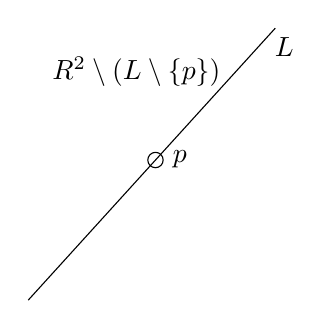
\begin{tikzpicture}[x=0.75pt,y=0.75pt,yscale=-1,xscale=1]
%uncomment if require: \path (0,232); %set diagram left start at 0, and has height of 232

%Straight Lines [id:da057879134343034266] 
\draw    (377,46) -- (258,177) ;

%Shape: Circle [id:dp27886143138574426] 
\draw   (315.6,109.5) .. controls (315.6,107.46) and (317.26,105.8) .. (319.3,105.8) .. controls (321.34,105.8) and (323,107.46) .. (323,109.5) .. controls (323,111.54) and (321.34,113.2) .. (319.3,113.2) .. controls (317.26,113.2) and (315.6,111.54) .. (315.6,109.5) -- cycle ;

% Text Node
\draw (326.4,103.8) node [anchor=north west][inner sep=0.75pt]   [align=left] {$p$};
% Text Node
\draw (268.4,58.8) node [anchor=north west][inner sep=0.75pt]   [align=left] {$\mathbb{R}^2 \setminus (L \setminus \{p\})$};
% Text Node
\draw (375.6,49.4) node [anchor=north west][inner sep=0.75pt]   [align=left] {$L$};
\end{tikzpicture}
\end{figure}

Comprobemos entonces que $\matheuler{T}_{Aspa}$ es topología:
\begin{enumerate}[label={(\arabic*)}]
\item Es inmediato comprobar que $\emptyset, X \in \matheuler{T}_{Aspa}$.
\item Comprobemos las uniones arbitrarias. Sean $U_i \in \matheuler{T}_{Aspa}$ con $i \in I$ arbitrario. Sea $(a,b) \in \bigcup_{i \in I} U_i$. Entonces, existe un $i_0 \in I$ tal que $(a,b) \in U_{i_0}$, luego $\exists \varepsilon > 0$ tal que $aspa((a,b), \varepsilon) \subset U_{i_0} \subset \bigcup_{i \in I} U_i$. Así, $\bigcup_{i \in I} U_i \in \matheuler{T}_{Aspa}$.
\item Comprobamos finalmente las intersecciones finitas. Sean $U, U' \in \matheuler{T}_{Aspa}$, y consideramos $(a,b) \in U \cap U'$. Entonces, $\begin{cases} \exists \varepsilon > 0 : aspa((a,b), \varepsilon) \subset U \\ \exists \varepsilon' > 0 : aspa((a,b), \varepsilon') \subset U' \end{cases}$. Si elegimos $\varepsilon_0 = \min \{\varepsilon, \varepsilon'\}$ se cumple que $aspa((a,b), \varepsilon_0) \subset U \cap U'$. Por tanto, $U \cap U' \in \matheuler{T}_{Aspa}$ y consecuentemente $\bigcap_{i \in I} U_i : I$ finito $\in \matheuler{T}_{Aspa}$.
\end{enumerate}
\end{ej}

\section{Número 1.8}
\begin{enun}
En $X = \mathbb{R}^2$ se consideran los subconjuntos $$G_t = \{(x,y) \in X : x > y + t\} \mbox{ con } t \in \mathbb{R}$$
Demostrar que estos subconjuntos, junto con $\emptyset$ y $X$, son los abiertos de una topología en $X$. ¿Es esto mismo cierto si $t \in \mathbb{N}$? ¿Y si $t \in \mathbb{Q}$?
\end{enun}
\begin{ej}
Antes de comprobar que la topología descrita $\matheuler{T}$ en efecto lo es, echamos un vistazo a la pinta que tienen los conjuntos $G_t$, lo cual nos ayudará a desarrollar una intuición de cómo proceder con la demostración.
$$\begin{tikzpicture}
\begin{axis}[
axis y line=middle,
axis x line=middle,
xticklabels={},yticklabels={},
grid = none, %major/minor
];
\addplot [
name path=A, very thick,black,mark=none, dashed,
domain=-3:12,samples=50,
] {x - 5};
\path    [name path=B] (-3,-8) --  (12,-8);
\addplot [teal, opacity=0.6] fill between [of=B and A,
        ];
\end{axis};
\end{tikzpicture}$$
Comprobemos entonces que $\matheuler{T}$ es una topología:
\begin{enumerate}[label={(\arabic*)}]
\item Por definición $\emptyset, X \in \matheuler{T}$.
\item Comprobemos las uniones arbitrarias. Sean $G_{t_i} \in \matheuler{T}$ con $i \in I$ arbitrario. Definimos $t^* = \inf t_i$, y observamos que 
$$\bigcup_{i \in I} G_{t_i} = \{(x,y) \in \mathbb{R}^2 : x > y + t_i\}$$
Distinguimos dos casos. En caso de que el ínfimo $t^*$ esté bien definido, esta unión es $G_{t^*}$, y por tanto es un abierto de $\matheuler{T}$. En el caso de que este ínfimo fuera $-\infty$, esta unión equivaldría a todo el conjunto $X$, que por definición también es abierto. Así, la unión arbitraria de elementos de $\matheuler{T}$ está en $\matheuler{T}$.
\item  Finalmente, comprobamos las intersecciones finitas. Sean $G_t, G_s \in \matheuler{T}$. Así, $G_t \cap G_s = \begin{cases} x - y > t \\ x - y > s \end{cases} \Rightarrow x - y > \max\{s,t\} = G_{\max\{s,t\}}$. Por tanto, $U \cap U' \in \matheuler{T}$ y consecuentemente $\bigcap_{i \in I} U_i : I$ finito $\in \matheuler{T}$.
\end{enumerate}
Contestamos las dos cuestiones siguientes:
\begin{itemize}
\item En el caso de que $t \in \mathbb{N}$, se siguen manteniendo las propiedades de topología, ya que si $t,t' \in \mathbb{N}$, entonces $\max \{t,t'\} \in \mathbb{N}$, y por tanto se conserva la propiedad de intersecciones finitas; y además, si tenemos una colección arbitraria $\{t_i\} \subset \mathbb{N}$, entonces sabemos que $\inf \{t_i\} \in \mathbb{N}$, luego también mantiene la propiedad de uniones arbitrarias. No obstante, la topología con los naturales tiene menos abiertos, y se dice menos fina o más gruesa.
\item En el caso de que $t \in \mathbb{Q}$, ya no nos encontramos ante una topología, pues el ínfimo de una sucesión de racional puede no ser racional, y por tanto no preservaría la propiedad de uniones arbitrarias.

Por ejemplo, si consideramos la sucesión $\displaystyle \lbrace - \left(1 + \frac{1}{n} \right)^n \} \longrightarrow -e$ obtenemos un contraejemplo.
\end{itemize}
\end{ej}
\chapter{Lista 2: Aplicaciones continuas}%
\label{cha:lista2}

\chapter{Lista 3: Construcción de topologías}%
\label{cha:lista3}

\chapter{Lista 4: Separación}%
\label{cha:lista4}

\chapter{Lista 5: Numerabilidad}%
\label{cha:lista5}

\chapter{Lista 6: Compacidad}%
\label{cha:lista6}

\chapter{Lista 7: Conexión}%
\label{cha:lista7}

\chapter{Lista 8: Conexión por caminos}%
\label{cha:lista8}

\chapter{Lista 9: Homotopía}%
\label{cha:lista9}

\chapter{Lista 10: Borsuk y sus variantes}%
\label{cha:lista10}
\end{document}
